% multiple1902 <multiple1902@gmail.com>
% intro.tex
% Copyright 2011~2012, multiple1902 (Weisi Dai)
% https://code.google.com/p/xjtuthesis/
%
% It is strongly recommended that you read documentations located at
%   http://code.google.com/p/xjtuthesis/wiki/Landing?tm=6
% in advance of your compilation if you have not read them before.
%
% This work may be distributed and/or modified under the
% conditions of the LaTeX Project Public License, either version 1.3
% of this license or (at your option) any later version.
% The latest version of this license is in
%   http://www.latex-project.org/lppl.txt
% and version 1.3 or later is part of all distributions of LaTeX
% version 2005/12/01 or later.
%
% This work has the LPPL maintenance status `maintained'.
%
% The Current Maintainer of this work is Weisi Dai.
%

\chapter{基于二叉树搜索的文字检测方法}
\echapter{Text detection based on Binary Tree Search}

    \section{问题的提出}
    \esection{Questions Posed}

    \section{方法原理与步骤}
    \esection{Principle and Summary of The Method}



    \section{候选文字行的提取}
    \esection{Candidate text line's extraction}

        \subsection{统计边缘响应}
        \esubsection{Static Skeleton Response}

        首先提出统计边缘响应方法,用以增强文本与背景之间的响应强度差异。给定如图\ref{fig.c4_static_skeleton_response}(a) 所示的场景文字图像$g$,计算其统计边缘响应$s$ 的方式如算法\ref{alg:c4_static_skeleton_response} 所示:

        \begin{algorithm} \renewcommand{\algorithmicrequire}{\textbf{输入:}}	\renewcommand{\algorithmicensure}{\textbf{输出:}}
    	\caption{统计边缘响应}
    	\label{alg:c4_static_skeleton_response}
    	\begin{algorithmic}[1]
    		\REQUIRE 输入的场景文字图像$g$
    		\ENSURE 图$g$相对应的统计边缘响应$s$
            \STATE 在图$g$上利用基于边缘骨架切割的文字检测子得到粗略的定位结果:文字定位包围框集合$B$ 及其相应的置信度分数集合$C$
    		\REPEAT
            \STATE $rs:=\left\{ b \times c  |\,b \in B, c \in C\right\}$
            \STATE $s:=s\cup rs,B:=B / b,C:=C / c$
            \UNTIL{$B=\varnothing$}
    	\end{algorithmic}
        \end{algorithm}

        其中$rs$指代的是响应小块,它的底面积是1 个定位包围框$b$,而高是$b$ 对应的置信度分数$c$。将所有的这些响应小块$rs$ 堆叠在一起,就构成了如图\ref{fig.c4_static_skeleton_response}(b) 所示的统计边缘响应$s$。

        \begin{figure}[!h]
        \begin{minipage}[t]{0.37\linewidth}
        \centering
        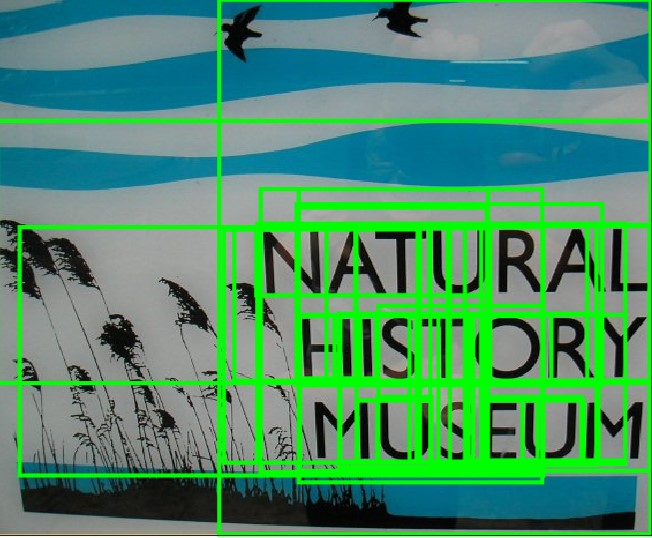
\includegraphics[width=\textwidth]{./figures/c4_img.jpg}
        \centerline{\small (a) 粗略定位结果}
        \end{minipage}
        \begin{minipage}[t]{0.35\linewidth}
        \centering
        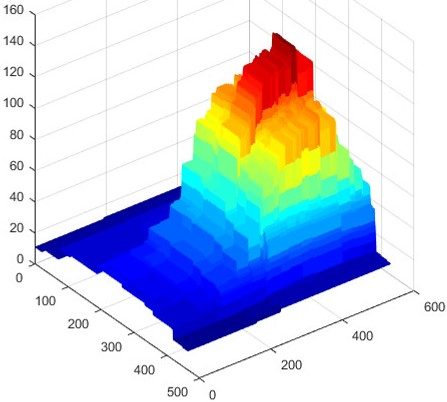
\includegraphics[width=\textwidth]{./figures/c4_static_skeleton_response.jpg}
        \centerline{\small (b) 统计边缘响应}
        \end{minipage}
        \begin{minipage}[t]{0.25\linewidth}
        \centering
        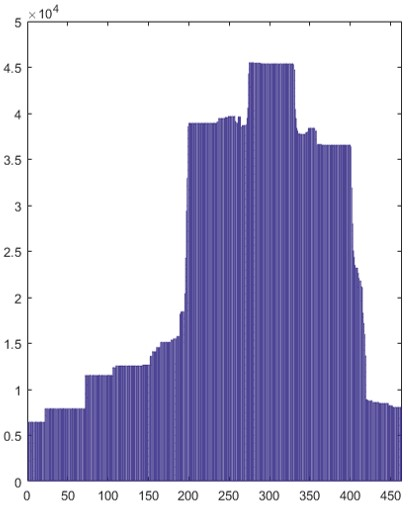
\includegraphics[width=\textwidth]{./figures/c4_horizontal_projection.jpg}
        \centerline{\small (c) 水平方向的映射}
        \end{minipage}
        \caption{在统计边缘响应中,文本区域与背景可以被区分开;而且通过后续的对统计边缘响应的水平映射操作,文本行也可以进一步区分开彼此}
        \label{fig.c4_static_skeleton_response}
        \end{figure}

        为了后续提取候选文本行的操作,首先要利用公式\ref{eq:c4_horizontal_projection} 来计算统计边缘响应$s$ 的横向投影$hp$,如图\ref{fig.c4_static_skeleton_response}(c) 所示。

        \begin{equation}
        hp= \left\{ \sum_{j=1}^w s_{ij} \, | \, i=1,2,...,h;j=1,2,...,w \right\},
        \label{eq:c4_horizontal_projection}
        \end{equation}

        其中,$h,w$分别是统计边缘响应$s$ 的高度和宽度。

        \subsection{候选文字行的生成}
        \esubsection{Text line's construction}

        在上1小节中得到了统计边缘响应$s$ 的横向投影$hp$, 它的数值如图\ref{fig.c4_candidate_line_construction}(a) 中的蓝色曲线所示,从中可看出候选文本行之间的响应有着明显的起伏变化。

        \begin{figure}[!h]
        \begin{minipage}[t]{0.32\linewidth}
        \centering
        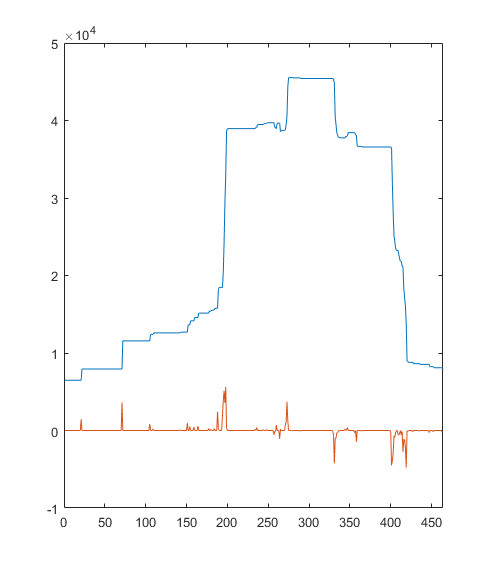
\includegraphics[width=\textwidth]{./figures/c4_gradient.jpg}
        \centerline{\small (a) 在水平映射图上的梯度}
        \end{minipage}
        \begin{minipage}[t]{0.32\linewidth}
        \centering
        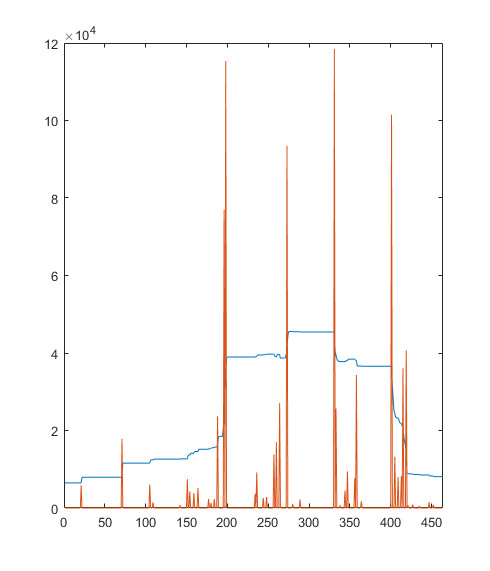
\includegraphics[width=\textwidth]{./figures/c4_unified.jpg}
        \centerline{\small (b) 梯度的取正和统一坐标}
        \end{minipage}
        \begin{minipage}[t]{0.32\linewidth}
        \centering
        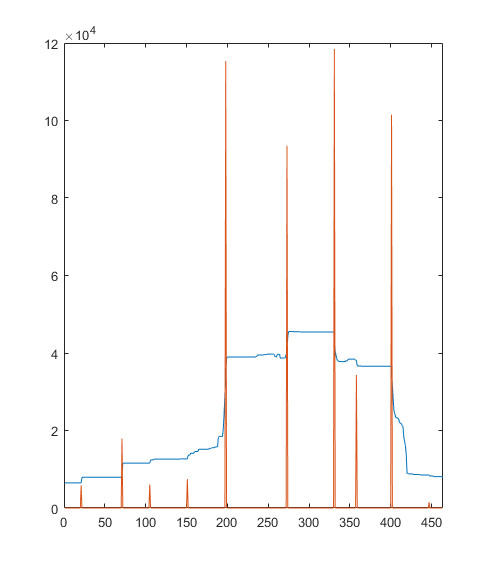
\includegraphics[width=\textwidth]{./figures/c4_nms.jpg}
        \centerline{\small (c) 梯度的非极大值抑制}
        \end{minipage}
        \caption{通过梯度计算和非极大值抑制操作来粗略定位文本行}
        \label{fig.c4_candidate_line_construction}
        \end{figure}

        为了确定候选文本行之间的分界线的具体位置,我们在统计边缘响应的横向投影$hp$上计算其梯度$g$,如图\ref{fig.c4_candidate_line_construction}(a) 中的脉冲状红线所示。梯度$g$表征着响应$hp$ 在某1 竖直位置上的变化程度:梯度$g$ 中的某1 脉冲状红线$l$ 的长度越大,就表明在红线$l$的附近越有可能存在着文字区域与背景区域之间的边界。而在梯度$g$中不存在脉冲红线的地方,意味着在这些区域的响应并没有发生突变,因此在$hp$ 上这些对应的位置上不存在文字区域与背景区域间的边界。

        为了便于观察和分析,首先对梯度值$g$取正,并将其提高至与$hp$统一的坐标内,如图\ref{fig.c4_candidate_line_construction}(b) 所示,这时得到的梯度值是$g$$'$。 最后在梯度值$g$$'$上执行非极大值抑制操作,由此消除掉绝大部分较小梯度值的无效脉冲状红线,并得到候选文本行集合$L$,而$L$ 由如图\ref{fig.c4_candidate_line_construction}(c) 中的$m$ 条红色候选文本行分割线组成。

    \section{二叉树型的文字行搜索空间的构建}
    \esection{Binary Tree-based search space's construction}

    将候选文本行集合$L$展现在场景文字原图上,如图\ref{fig.c4_binary_tree_construction}(b) 所示。$L$ 由$m$ 条红线$l_i, i=1,2,...,m$ 构成,这些红线是候选文本行分割线,并且在场景文字原图上分割出$m+1$个候选文本行条带,而这些文本行条带就是任两个相邻红线$l_i$和$l_{i+1}$ 之间的图像区域。那么现阶段的任务是,将所有候选文本行条带区域的排练组合作为1 个搜索空间,然后从中搜寻出最优的文本行条带组合,而这些条带区域能恰如其分地覆盖住文字所在的图像区域。

    \begin{figure}[!h]
    \centering
    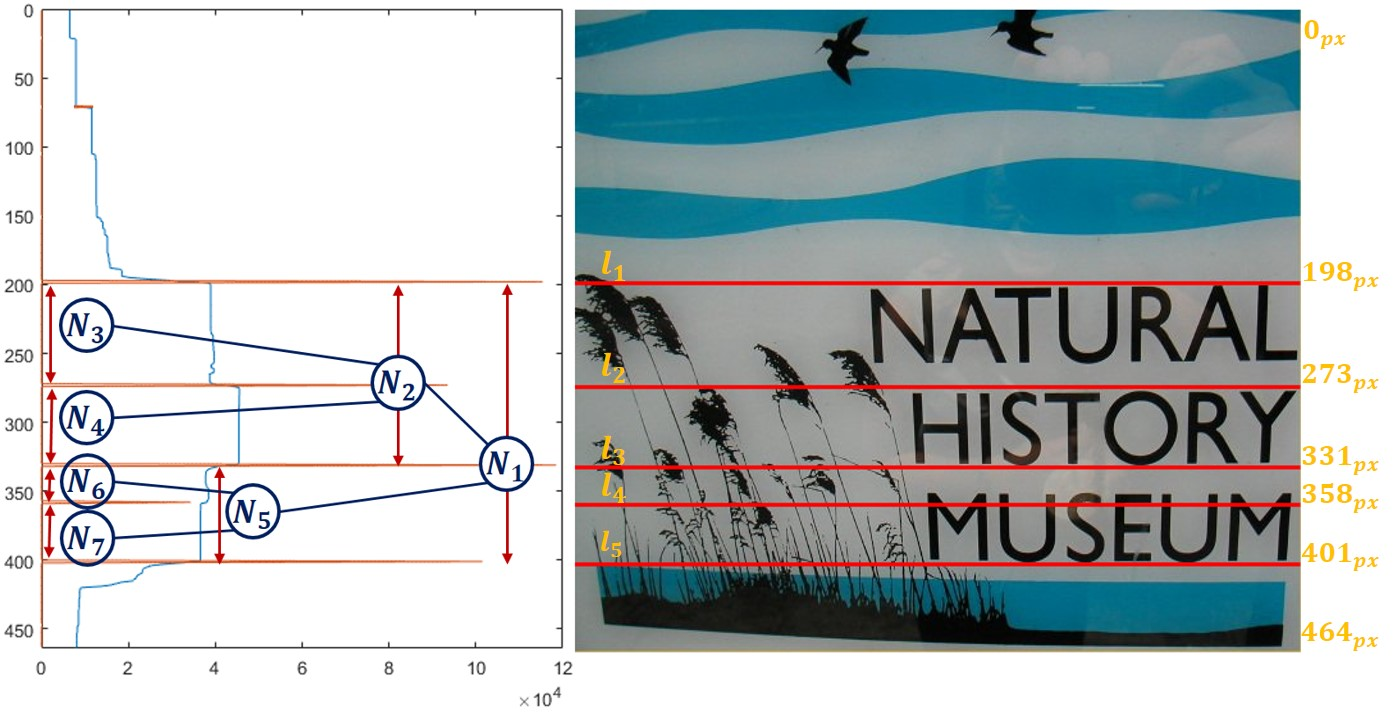
\includegraphics[width=\textwidth]{./figures/c4_binary_tree_construction.jpg}
    \begin{minipage}[t]{0.40\linewidth}
    \centerline{\small (a)二叉树型搜索空间}
    \end{minipage}
    \begin{minipage}[t]{0.51\linewidth}
    \centerline{\small(b)在场景图像中的候选文本行}
    \end{minipage}
    \caption{从候选文本行中建立起代表搜索空间的二叉树型数据结构}
    \label{fig.c4_binary_tree_construction}
    \end{figure}

    假设红色分割线$l_i$有2个属性:距离$ld_i$ 和置信度$lc_i$。 其中属性$ld_i$ 指代的是从图像顶部到分割线$l_i$ 位置的距离,例如在图\ref{fig.c4_binary_tree_construction}(b) 中,$ld_3=331_{px}$就是指从图像顶部到线$l_3$的距离有331 个像素大小。而$lc_i$ 是分割线$l_i$的置信度,其数值是由$l_i$ 的梯度值归一化得到的,例如在图\ref{fig.c4_binary_tree_construction}(b) 中,$lc_3=0.987$ 表征的是$l_3$是文本行之间分割边界的可能性非常大。

    然后假设我们要构建的二叉树型搜索空间$N$是由一些结点$n$ 构成的。其中任一结点$n_i$有2 个对应的属性:结点代表的图像区域范围$nr_i$,以及结点的数值$nv_i$。以图\ref{fig.c4_binary_tree_construction}(a) 为例,节点$n_5$ 所代表的文本行区域范围是从线$l_3$ 到$l_5$之间的区域,而$n_5$ 的值是由$l_4$ 的置信度值$lc_4$ 赋予的。

    在明确候选文本行分割线$L$,以及二叉树型搜索空间$N$ 中各变量的含义后,由$L$构建$N$ 的过程如算法\ref{alg:c4_build_binary_tree} 所示:

    \begin{algorithm}[!h]
	\renewcommand{\algorithmicrequire}{\textbf{输入:}}
	\renewcommand{\algorithmicensure}{\textbf{输出:}}
	\caption{递归地建立二叉树型搜索空间}
	\label{alg:c4_build_binary_tree}
	\begin{algorithmic}[1]
		\REQUIRE 分割线 $L$ 的距离 $LD=\left\{ld_1,ld_2,...,ld_m\right\}$ 和置信度$LC=\left\{lc_1,lc_2,...,lc_m\right\}$
		\ENSURE 二叉树型搜索空间 $N$ 的结点范围 $NR=\left\{nr_1,nr_2,...,nr_{2m-3}\right\}$, 和结点的值 $NV=\left\{nv_1,nv_2,...,nv_{2m-3}\right\}$
      \STATE 初始化: \\
      \STATE \quad $i=0, \quad BuildBinaryTree(i,LD,LC)$
      \STATE function $BuildBinaryTree(i,LD,LC)$
        \\\STATE \quad $i=i+1$
        \\\STATE \quad $if \quad length(LD)==2 \quad then$
        \\\STATE \qquad $nr_{i}=[LD[1],LD[2]], nv_{i}=0$
        \\\STATE \qquad $return$
        \\\STATE \quad $end \ if$
        \\\STATE \quad $nr_{i}=[LD[1],LD[end]], nv_{i}=max(LC)$
        \\\STATE \quad $//$假设$LC$中的最大值是$lc_t$,其中$t$ 是$lc_t$ 的索引
        \\\STATE \quad $//$在索引$t$处将$L$分裂成左子集和右子集
        \\\STATE \quad $LD_{l}=\left\{LD[1],...,LD[t]\right\}, LC_{l}=\left\{LC[1],...,LC[t]\right\}$
        \\\STATE \quad $BuildBinaryTree(i,LD_{l},LC_{l})$
        \\\STATE \quad $LD_{r}=\left\{LD[t],...,LD[end]\right\}, LC_{r}=\left\{LC[t],...,LC[end]\right\}$
        \\\STATE \quad $BuildBinaryTree(i,LD_{r},LC_{r})$
      \STATE end function
	\end{algorithmic}
    \end{algorithm}

    那么,通过算法\ref{alg:c4_build_binary_tree} 从$L$ 中构建好的二叉树型搜索空间$N$就将存储在如图中的表格内。下一节,将介绍从搜索空间$N$ 中搜寻出最优文本行定位的搜索策略。

    \section{搜索最优的文字行定位}
    \esection{Searching the optimal text detection}

        \subsection{搜索路径}
        \esubsection{Searching the paths}

        给定二叉树型搜索空间$N$,假设$N$是由$m$ 个结点$n$ 构成,那么通过算法\ref{alg:c4_binary_tree_search},就可搜索出路径$P={p_1,p_2,...,p_{(m-1)/2}}$。 路径中的每个$p_i \in P$ 都是1个3元组:包含了父亲结点$np_i$,左子结点$nl_i$和右子结点$nr_i$。

        \begin{algorithm}[!h]
    	\renewcommand{\algorithmicrequire}{\textbf{输入:}}	
        \renewcommand{\algorithmicensure}{\textbf{输出:}}
    	\caption{从二叉树型搜索空间中找到最优路径}
    	\label{alg:c4_binary_tree_search}
    	\begin{algorithmic}[1]
    		\REQUIRE 二叉树型搜索空间 $N=\left\{n_1,n_2,...,n_m\right\}$, 其中每个结点$n_x \in N$有其相应的属性: 范围$nr_x$ 和值$nv_x$
    		\ENSURE 搜索到的路径 $P=\left\{p_1,p_2,...,p_{(m-1)/2}\right\}$, 其中每条路径$p_{i} \in P$ 包含结点三元组$p_{i}=\left\{np_{i},nl_{i},nr_{i}\right\}$

          \STATE 初始化: $idx=0$
          \FOR{$i=1$ to $(m-1)/2$}

          \FOR{$j=1$ to $m$}
          \IF{$nv_j$ == $leastPositive(NV)$}
          \STATE $np_i = n_j, nv_j = 0, idx = j$
          \ENDIF

          \IF{$nr_j[1]$ == $nr_{idx}[1]$ and $nv_j$ == $0$}
          \STATE $nl_i = n_j, nv_j = -1$
          \ENDIF

          \IF{$nr_j[2]$ == $nr_{idx}[2]$ and $nv_j$ == $0$}
          \STATE $nr_i = n_j, nv_j = -1$
          \ENDIF

          \ENDFOR

          \STATE $p_{i}$ = $\left\{ np_{i},nl_{i},nr_{i} \right\}$

          \ENDFOR
    	  \end{algorithmic}
        \end{algorithm}

        算法\ref{alg:c4_binary_tree_search} 的具体过程如下所述:根据二叉树的性质,如果二叉树$N$ 中存在$m$ 个结点,那么算法\ref{alg:c4_binary_tree_search} 就要迭代执行$(m-2)/2$ 次。在第$i$次迭代中:首先将具有最小正数值$nv_j \in NV$ 的结点$n_j \in N$,赋予路径三元组中的父亲结点$np_i$,并将$nv_j$ 设为0,从而使结点$n_j$转换为叶子结点;然后在二叉树$N$ 中寻找能赋予路径三元组中左子结点$nl_i$的1 个结点$n_x$,该结点必须满足下述条件:$n_x$的范围的左边界$nr_x$[1]须和$n_j$ 的范围的左边界$nr_j$[1] 相等,且其值$nv_x$ 须为0。那么找到满足要求的结点$n_x$,并将其赋予$nl_i$。 紧接着将该结点的值$nv_x$ 设为-1,这意味着结点$n_x$ 已被标注为``已处理'',也就是说结点$n_x$ 不会在算法的下一轮迭代中被考虑;类似地,搜索到$n_t$并将其赋予路径三元组中的右子结点$nr_i$,然后将$n_t$ 的值改为-1。

        以上过程是算法\ref{alg:c4_binary_tree_search} 的第i 次迭代。那么经过$(m-1)/2$次迭代后,包含$(m-1)/2$ 个三元组$p$的路径集合$P$就被构建了出来。

        \begin{figure}[!h]
        \centering
        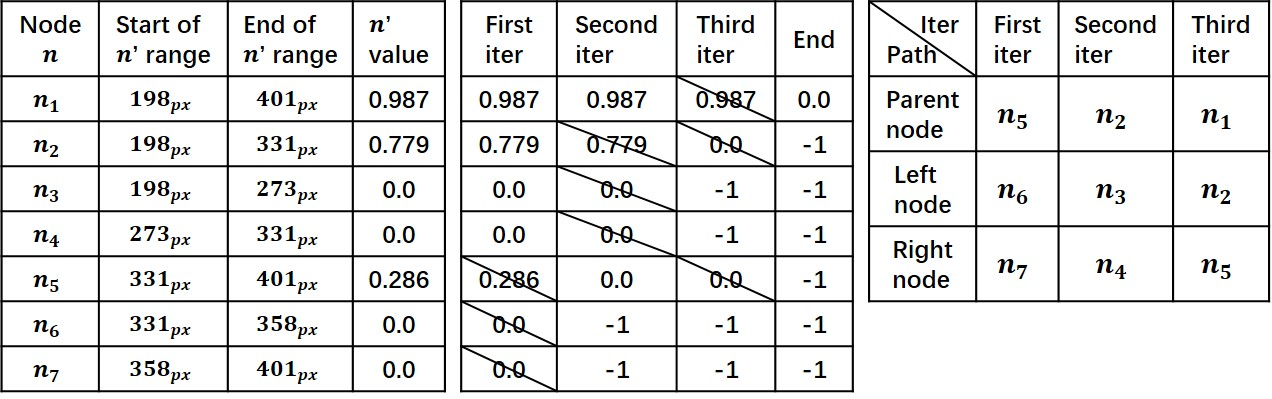
\includegraphics[width=\textwidth]{./figures/c4_bianry_tree_search.jpg}
        \begin{minipage}[t]{0.33\linewidth}
        \centerline{\small (a) 存储二叉树型搜索空间的表格}
        \end{minipage}
        \begin{minipage}[t]{0.33\linewidth}
        \centerline{\small(b)二叉树搜索算法的迭代过程}
        \end{minipage}
        \begin{minipage}[t]{0.26\linewidth}
        \centerline{\small(C)搜索到的路径结果}
        \end{minipage}
        \caption{1个从二叉树型搜索空间中找到最优路径的示例}
        \label{fig.c4_bianry_tree_search}
        \end{figure}

        为了更直观地理解算法\ref{alg:c4_binary_tree_search}:从二叉树型搜索空间中找到最优路径的算法,这里用图\ref{fig.c4_bianry_tree_search} 所示的例子加以阐述。首先图\ref{fig.c4_bianry_tree_search}(a) 中的表格存储的是代表候选文本行搜索空间的二叉树$N$,且在这个例子中,$N$含有7个结点;然后采用算法\ref{alg:c4_build_binary_tree} 在$N$上进行搜索,算法将会执行$(7-1)/2=3$ 次迭代,每次迭代的具体过程如图\ref{fig.c4_bianry_tree_search}(b) 所示;最后,算法的每次迭代,都会生成1 个对应的结点三元组。那么经历3 次迭代后,就会得到如图\ref{fig.c4_bianry_tree_search}(c) 所示的路径集合,即为算法\ref{alg:c4_binary_tree_search} 的搜索结果。

        \subsection{搜索策略}
        \esubsection{Searching strategies}
        \label{sec.c4_searching strategies}

        得到路径集合$P$后,在$P$上执行搜索策略,以得到最优的文本行定位。以图\ref{fig.c4_search_strategy}(a) 中的1 个被搜索到的路径三元组$p_i$为例,$p_i=\left\{np_i,nl_i,nr_i\right\}=\left\{n_5,n_6,n_7\right\}$。 那么对$p_1$的决策将在下列的3 项策略中选出并仅选出1 种:

        (1)保留父亲结点$n_5$ 所代表的融合的文本行区域,而剪掉子结点$n_6$和$n_7$ 各自所代表的分离的文本行区域;

        (2)仅保留子结点$n_7$ 所代表的那部分单独的文本行区域,而剪掉父亲结点$n_5$ 所代表的融合的文本行区域以及子结点$n_6$ 所代表的单独的文本行区域;

        (2)仅保留子结点$n_6$ 所代表的那部分单独的文本行区域,而剪掉父亲结点$n_5$ 所代表的融合的文本行区域以及子结点$n_7$ 所代表的单独的文本行区域;

        对上述3种策略的选择过程是基于\ref{fig.c4_search_strategy}(b) 所示的2 阶段的判别步骤,而判别的依据是结点$n_6,n_7$ 以及$n_5$ 的识别成绩高低。这里采用的识别模型是Jaderberg等\cite{Jaderberg2016Reading} 的深度学习文字识别网络。我们按照结点的范围区域$nr$ 来截取出包含候选文本行的图块,将其输入文字识别网络,以得到该结点所代表文本行区域的识别成绩,并将其赋予结点的值$nv$。

        \begin{figure}[!h]
        \centering
        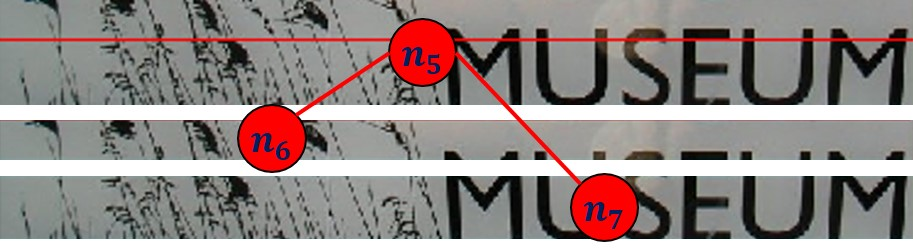
\includegraphics[width=\textwidth]{./figures/c4_search_strategy1.jpg}
        \centerline{\small (a) 1个被搜索到的路径三元组:其中每个结点代表1个候选文本行区域 }
        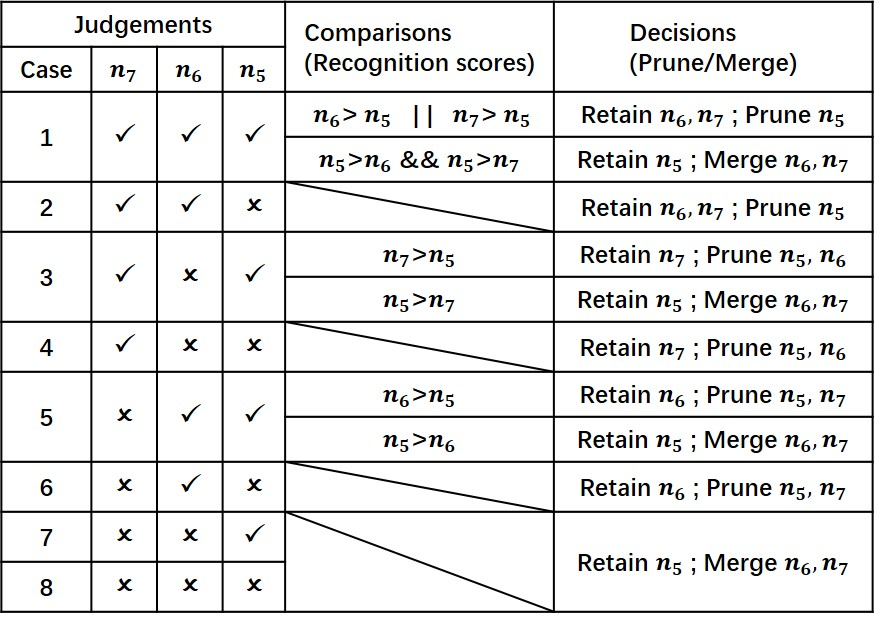
\includegraphics[width=\textwidth]{./figures/c4_search_strategy2.jpg}
        \centerline{\small (b) 对路径三元组的剪枝或融合策略}
        \caption{ 1个搜索策略的示例}
        \label{fig.c4_search_strategy}
        \end{figure}

        具体的2阶段判决过程如图\ref{fig.c4_search_strategy}(b) 所示:首先在第1 阶段的判断过程中,结点$n_i$ 所代表的文字行区域要根据该结点的识别成绩值$nv$ 来进行而分类:如果$nv_i>0$,那么结点$n_i$ 所代表的区域被判定为文本行区域,并用对号标记;而如果$nv_i<0$,那么结点$n_i$ 所代表的区域被判定为非文本区域,并用错号标记。通过上述对3 个结点的二分类判断后,就会在$8=2^3$种情况中只选定1种情况条目进行后续的处理。然后在第2阶段的比较过程中,拿选定情况条目中的结点值$nv$进行对比,以此得到最终的决策结果。用图\ref{fig.c4_search_strategy}(b) 举例来说:假如$n_7$ 和$n_5$都被判定为文本,而$n_6$被判定为非文本,那么根据第1阶段的判定过程,选定情况条目3;然后在情况条目3中,经过第2 阶段比较过程,发现结点值$nv_5>nv_7$,那么得到最终的决策结果是:保留父亲结点$n_5$代表的融合的文本行区域,而剪掉子结点$n_6$ 和$n_7$ 各自所代表的分离的文本行区域。

        同理,下1条路径三元组$p_{i+1}=\left\{np_{i+1},nl_{i+1},nr_{i+1}\right\}$ 依然会在2阶段判决过程中得到自己相应的决策结果。那么重复该搜索策略,直到路径集合$P$ 中的所有路径三元组都经过处理而获得决策结果。最终,就获得了从二叉树型搜索空间中搜索得到的最优文本行定位结果。

    \section{实验和结果分析}
    \esection{Experimental Results}

        \subsection{实验数据集与评价标准}
        \esubsection{Data-set and Evaluation Protocol}

        为了验证本章提出的文字检测方法的效果和性能,我们将这个方法在ICDAR 2003(IC03),ICDAR 2011(IC11)以及ICDAR 2013(IC13)测试数据集上都运行并得到了结果。其中IC03,IC11和IC13各包含251,255及233张标注了文本的自然场景图像。这些测试数据集因其字体、颜色、尺度和光照的不同和变化而极具挑战性。

        最后将本方法与其它先进的文字检测和识别方法在谷歌街景数据集(Google Street View Text dataset,简称为SVT)进行了对比实验。SVT 文字测试集包含249张包含文字的街景图像。这些图像大多是模糊、光照不均的,并且数据集中的文字并未完全标注过,因此该文字检测数据集也充满了挑战。

        用以评价文字检测效果的标准依然是Wolf 等\cite{Wolf2006Object}提出的Object/area graphs 方法。其中对文字检测查全和查准率的计算公式如下所示:

        $recall = \frac {\sum_{i=1}^{|G|}Match_G(G_i,D,t_r,t_p)} {|G|}  ,   precision =\frac {\sum_{j=1}^{|D|}Match_G(D_j,G,t_r,t_p)} {|D|}$

        而文字检测的$f$值是查全recall和查准precision的均值。

        此外本章提出的方法还与其它方法在各场景文字图片数据集上进行了识别成绩的对比实验。用以验证识别效果的评判标准来自Wang\cite{Wang2012End}的方法。识别结果包含所有的拉丁文字,但是忽略那些不足3个字符长度的单词。只有当检测到的1个候选文字的包围框与文字定位结果真值(ground truth) 的重叠率(Interaction over Union,简称为IoU)超过50\% 时,该候选文字的识别成绩才被认为是有效的。

        \subsection{实验结果与分析}
        \esubsection{Experimental Results and Analysis}

        如表格\ref{tab.c4_icdar13}所示,在自然场景文字图片数据集ICDAR 2013上,一些最先进的文字检测方法例如Cho\cite{Cho2016Canny} 的方法取得了81.1\%的检测F 值,而我们的方法的检测F 值能达到82.3\%。其中,本章提出的方法取得了75.5\% 的查准率以及高达89.2\% 的查全率。本方法的查全率远高于其它先进的文字检测方法的查全率,原因就在于文本行的二叉树型搜索空间的建立,以及最优文本行搜索策略的执行。

        值得注意的是本章提出的方法是一种快速的文字检测算法,与Tian\cite{Tian2016Text} 的基于CNN的文字检测子相比,本方法消耗的是极小的计算量和时间。在ICDAR 2013的数据集中,平均的图像尺寸大约是1200乘以900个像素大小。而本章提出的方法平均处理一张图像大概只用0.76 秒左右,这其中包括了基于边缘骨架的文字检测子,统计边缘响应以及基于二叉树型搜索空间搜索的文本行优化等步骤的全过程。此外,与我们在上一章提出的方法即He\cite{He2017scene}的文字检测方法相比,本章新提出的基于二叉树搜索的文本行矫正方法,又使F 值提升了近2\%,由此证明该方法的确增强了文字检测的查全效果及查准效果。

        \begin{table}[!h]
        \centering
        \caption{在ICDAR 2013上的文字检测效果(\%)}
        \begin{tabular}{p{0.25\textwidth}|p{0.25\textwidth} p{0.25\textwidth} p{0.13\textwidth}}
        \hline
        方法 & 查全R & 查准P & F值 \\
        \hline
        \textbf{Proposed} & \textbf{89.2} & \textbf{75.5} & \textbf{82.3}\\
        He\cite{He2017scene} & 76.2 & 86.7 & 81.1 \\
        Cho\cite{Cho2016Canny} & 78.4 & 86.2 & 82.1 \\
        Tian\cite{Tian2016Text} & 75.8 & 85.1 & 80.2 \\
        Zhu\cite{Zhu2016Text} & 75 & 85 & 79 \\
        Gupta\cite{Gupta2016Synthetic} & 66.30 & 94.80 & 78.00 \\
        Pham\cite{Pham2016Robust} & 65.11 & 83.98 & 75.89 \\
        Neumann\cite{Neumann2012Real} & 64.84 & 87.51 & 74.49 \\
        \hline
        \end{tabular}
        \label{tab.c4_icdar13}
        \end{table}

        如表\ref{tab.c4_icdar11}所示,在ICDAR 2011 文字测试数据集上,本章提出的基于二叉树搜索的文字检测方法与上一章提出的He\cite{He2017scene}的方法,以及其它最先进的的文字检测方法如Cho\cite{Cho2016Canny}、Sung\cite{Sung2015Scene} 等的方法都进行了字符提取数目和检出率的量化对比。从实验结果上来看,本章提出的方法可以在获得最高文字检出率的同时,保证提取的字符数目最少。该实验说明表明,相对于其它先进文字检测方法而言,本章方法都达到更优的文字查全和查准效果的折衷。

        \begin{table}[!h]
        \centering
        \caption{在ICDAR 2011测试集上对于字符提取数目和检出率的测评}
        \begin{tabular}{p{0.33\textwidth}|p{0.33\textwidth} p{0.25\textwidth}}
        \hline
        方法 & 候选字符数目 & 检出率 \\
        \hline
        All ERs & 6,051,331 & 0.966 \\
        Matas\cite{Matas2004Robust} & 39,762 & 0.539 \\
        Sung\cite{Sung2015Scene} & 93,357 & 0.877  \\
        Cho\cite{Cho2016Canny} & 8,121 & 0.874 \\
        He\cite{He2017scene} & 8,231 & 0.879 \\
        \hline
        \textbf{Proposed} & \textbf{7,137} & \textbf{0.892} \\
        \hline
        \end{tabular}
        \label{tab.c4_icdar11}
        \end{table}

        图\ref{fig.c4_recall_proposals}展示的是在本章提出方法的各阶段中,字符检出率与候选字符提取数目的关系折线图。与上一章提出的He\cite{He2017scene} 的方法相比,本章的方法在基于边缘骨架切割的文字检测子的基础上,融入了基于二叉树型搜索空间搜索的文本行定位优化方法。其中,基于二叉树搜索的文本行矫正进一步减少了非文字候选字符的提取数目,同时却提升了候选字符的查全效果。因此本章方法相对上一章方法,字符检出率增高2\%,且提取的候选字符数目能降低10\%。

        \begin{figure}[!h]
        \centering
        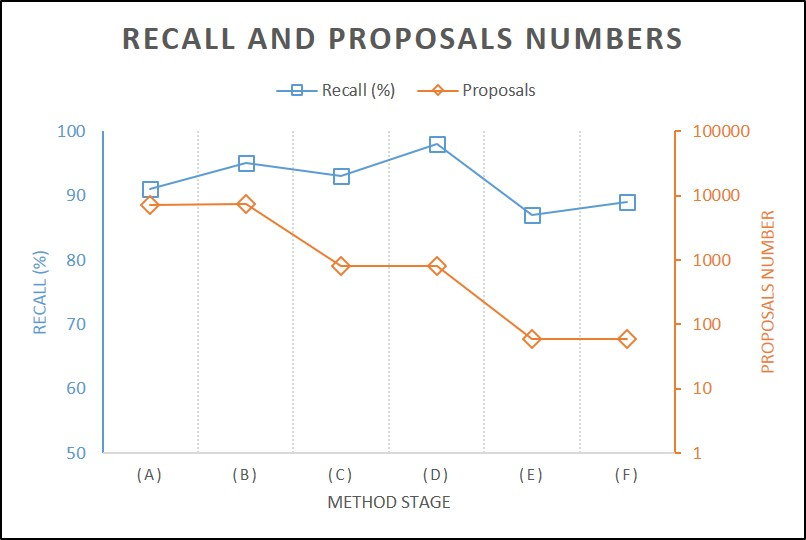
\includegraphics[width=\textwidth]{./figures/c4_recall_proposals.jpg}
        \caption{在ICDAR 2011 数据集上,本方法在各阶段中的文字检测查全与候选字符提取数目间的关系折线图: (a) 候选文字边缘骨架提取, (b) 文字边缘骨架切割, (c) 文字边缘骨架过滤, (d) 候选文本行定位, (e)非极大值抑制, (f) 基于二叉树搜索的文本行优化。}
        \label{fig.c4_recall_proposals}
        \end{figure}

        在第\ref{sec.c4_searching strategies}节基于二叉树搜索的文本行优化的搜索策略中,我们详细探讨过自然场景文字检测与识别之间的紧密关系。其中,依据文字识别的成绩,文字检测的结果才能更准确的定位到文本行的位置。而反过来,更准确的文字检测结果,也会进一步的增强文字识别的精度。

        因此,我们也将本章提出的方法与其他方法在各场景文字图片数据集上做了识别成绩的对比实验,如表\ref{tab.c4_recognition} 所示。在所有的数据集上,本章提出的方法的端对端识别成绩都高于其它所有方法。在SVT-50数据集上,由Jaderberg\cite{Jaderberg2016Reading}提出的端对端识别模型获得了P/R/F(查准/查全/F值)分别为0.85/0.68/0.76的识别分数,而本章方法在这个成绩基础上继续提升5\%从而达到0.86/0.67/0.77的识别成绩。同样在IC03 的各种词典配置的数据集上(IC03-50,IC03-FULL 和 IC03),本章方法相对于其它先进方法对F值的提升均在2\%左右,最终达到P/R/F分别为0.96/0.87/0.92的识别分数。

        \begin{table*}[!h]
        \centering
        \caption{本章提出方法与其它先进方法的端对端文字识别成绩}
        \begin{tabular}{l|l l l l l l l}
        \hline
        方法 & IC03-50 & IC03-FULL & IC03 & SVT-50 & SVT & IC11 & IC13  \\
        \hline
        Neumann\cite{Neumann2010A} & -- & -- & 41 & -- & -- & -- & -- \\
        Wang\cite{Wang2012End} & 68 & 51 & -- & 38 & -- & -- & -- \\
        Wang\cite{Wang2012End} & 72 & 67 & -- & 46 & -- & -- & -- \\
        Matas\cite{Matas2014Scene} & -- & -- & -- & -- & -- & -- & 45 \\
        Alsharif\cite{Alsharif2013End} & 77 & 70 & 63 & 48 & -- & -- & -- \\
        Jaderberg\cite{Jaderberg2014Deep} & 80 & 75 & -- & -- & 56 & -- & -- \\
        Jaderberg\cite{Jaderberg2016Reading} & 90 & 86 & 78 & 76 & 53 & 76 & 76 \\
        He\cite{He2017scene} & 91 & 85 & 78 & 77 & 53 & 75 & 77 \\
        \textbf{Proposed} & 92 & 86 & 79 & 77 & 55 & 78 & 79 \\
        \hline
        \end{tabular}
        \label{tab.c4_recognition}
        \end{table*}

        对于表\ref{tab.c4_recognition}中那些不含词典(lexicon) 的文字图片数据集,我们同样给出了本章提出方法与其它先进方法的识别成绩对比。可以预料的一点是,当数据集缺失词典的限制时,所有方法的F值都遭受了损失。但从实验结果来看,本章提出方法的识别成绩仍然高于其它的方法。表中显示在SVT-50和SVT数据集上,本方法分别获得77\%和55\%的识别成绩,均高于其他所有方法。而与上一章提出的方法进行对比,发现在SVT数据集上有一定的提升,而在ICDAR11和ICDAR13数据集上提升了近3\%,这也表明了基于二叉树搜索的文本行定位优化以及识别可以很好的处理定位不甚准确的单词,因此可以进一步提高文字检测和识别效果。一些在ICDAR 2013数据集上的检测结果如图\ref{fig.c4_results_ic13}所示,而在SVT数据集上的结果样例如图\ref{fig.c4_results_svt}所示。从结果图可见,本章提出方法可以检测有粘连、模糊、过度曝光等问题的文字。
        
        \begin{figure}[!h]
        \centering
        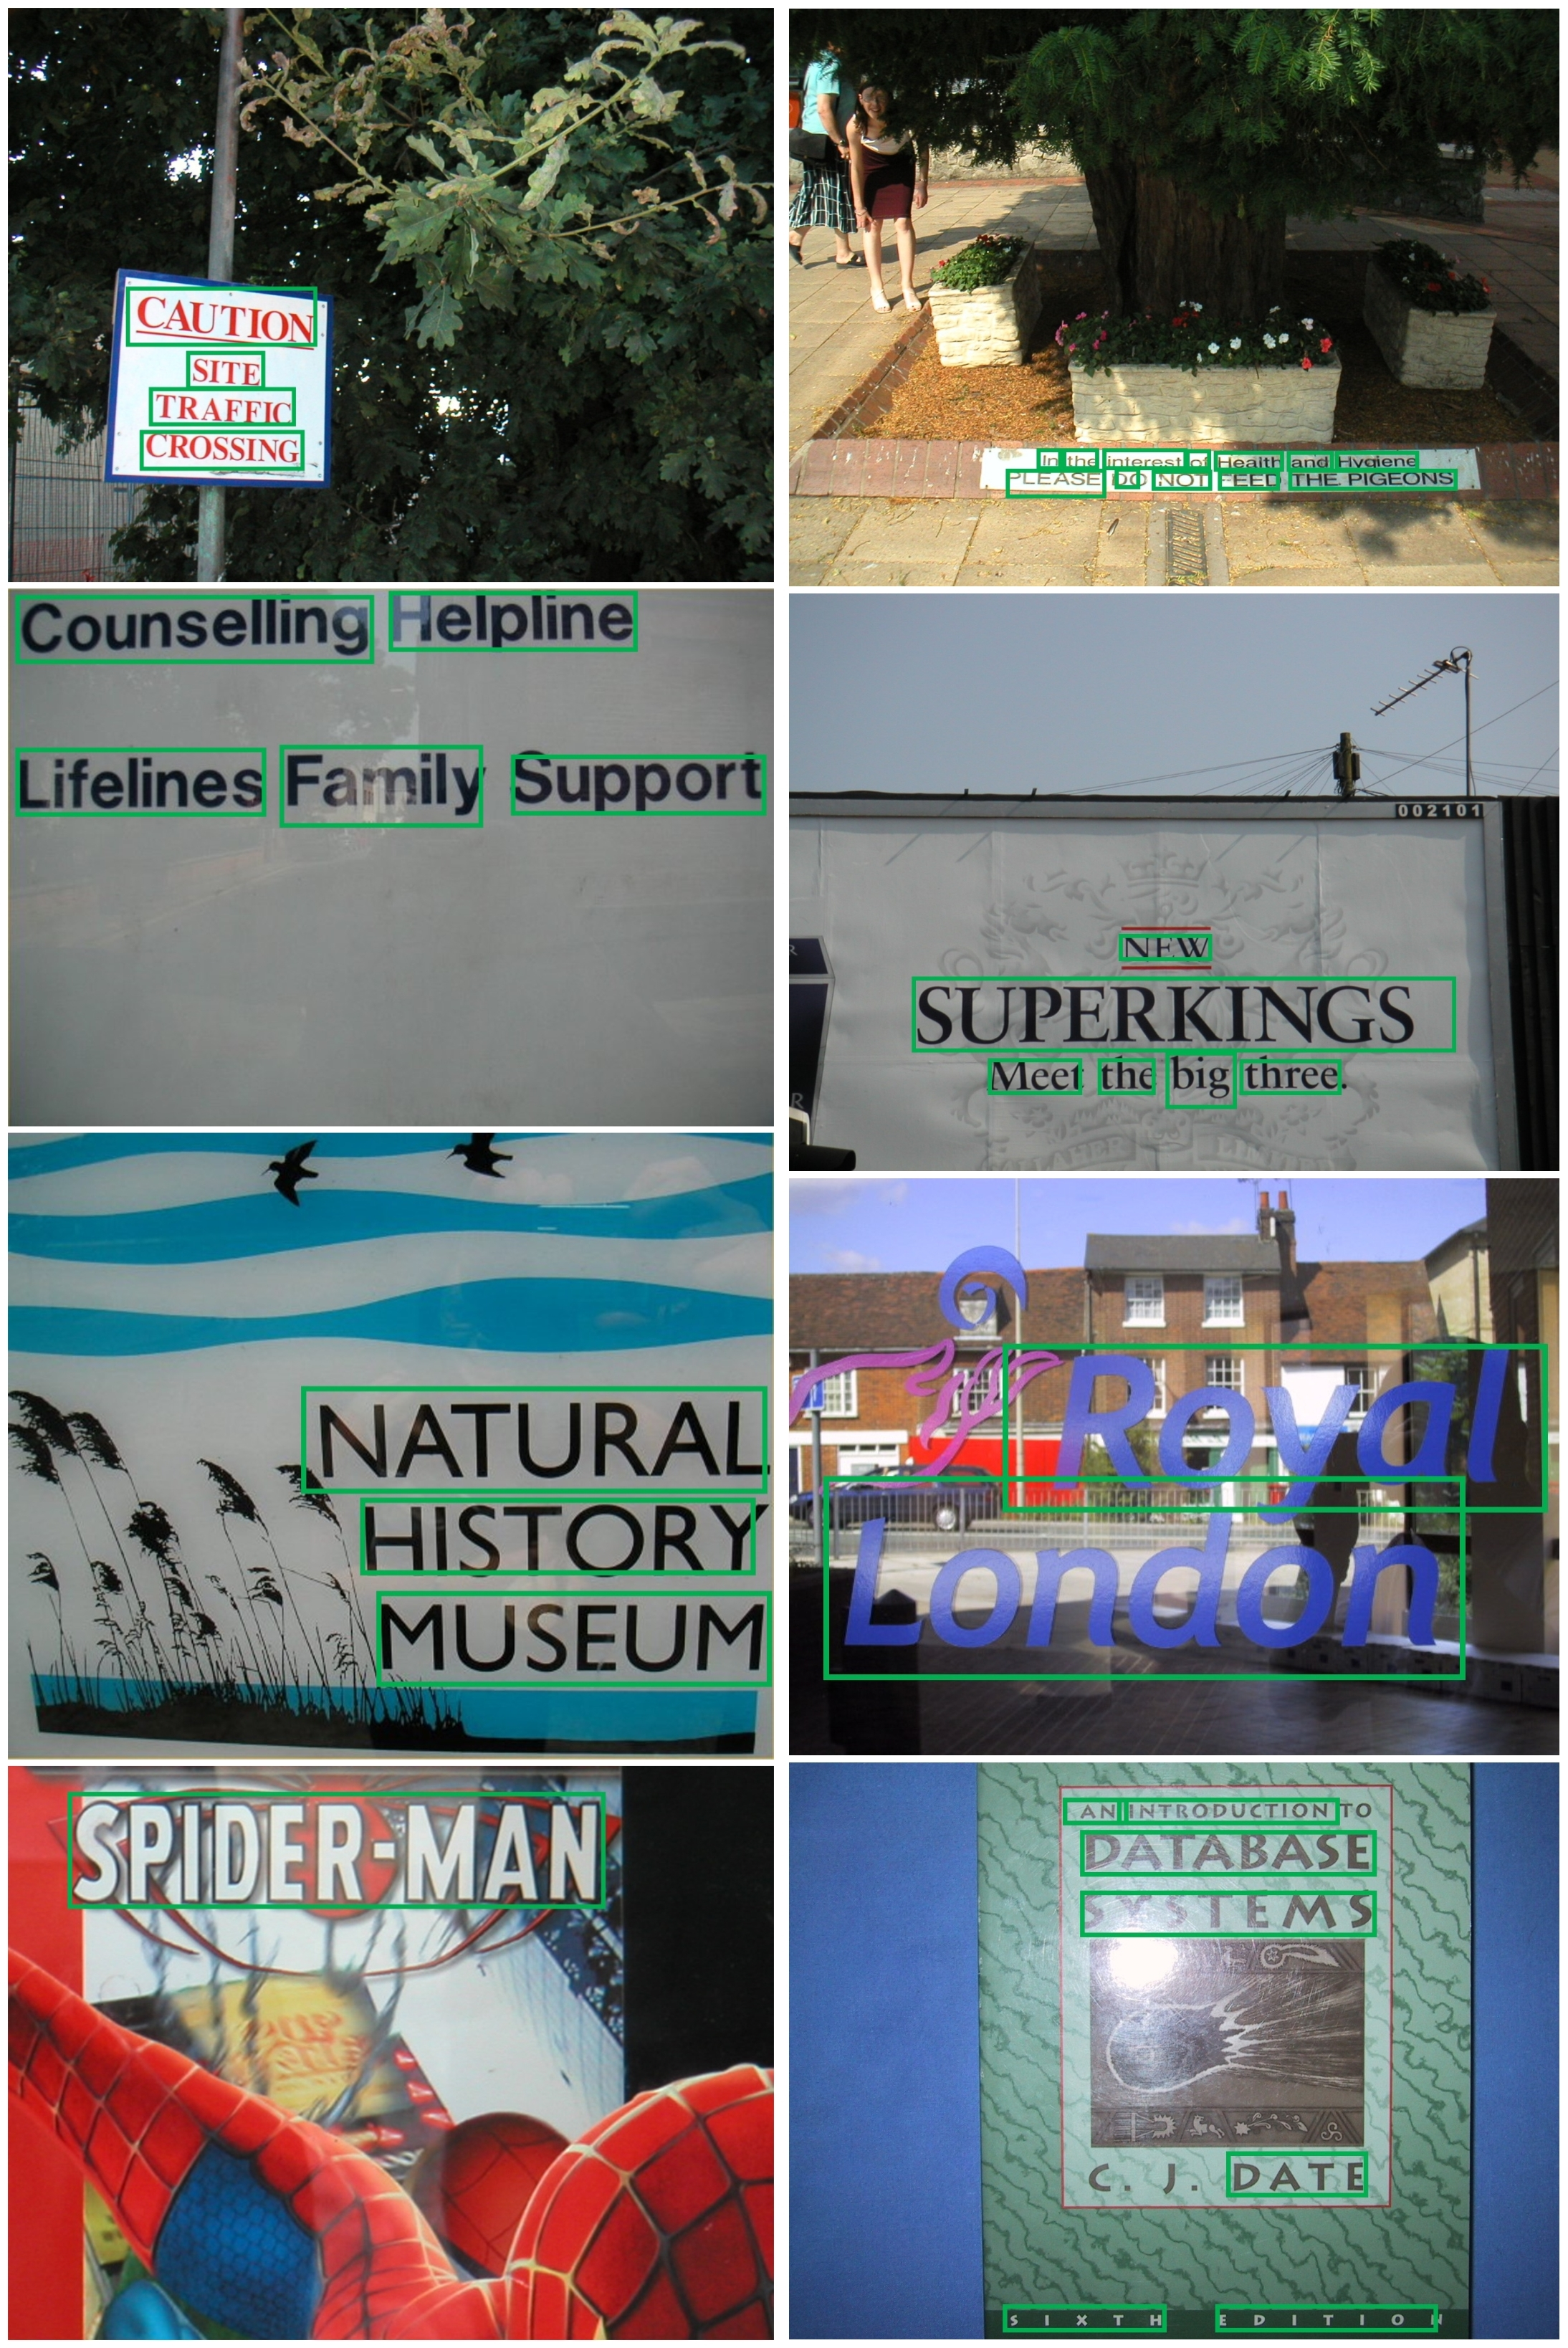
\includegraphics[width=\textwidth]{c4_results_ic13.jpg}
        \caption{ICDAR2013 上的测试结果示例}
        \label{fig.c4_results_ic13}
        \end{figure}

        \begin{figure}[!h]
        \centering
        \includegraphics[width=\textwidth]{c4_results_svt.jpg}
        \caption{SVT数据集上的测试结果示例}
        \label{fig.c4_results_svt}
        \end{figure}


    \section{本章小结}
    \esection{Brief Summary}


